\documentclass[11pt]{article}

% ── Preamble ──────────────────────────────────────────────────────────────────
\usepackage[margin=1in]{geometry}
\usepackage{microtype}
\usepackage{mathtools, amssymb, amsthm}
\usepackage{graphicx, booktabs}
\usepackage{enumitem}
\usepackage{csquotes}
\usepackage[dvipsnames]{xcolor}
\usepackage{hyperref}
\usepackage{cleveref}
\usepackage{caption}

% Search both paper/ directory and repo root for figures
\graphicspath{{./}{../}}

% Hyperref setup
\hypersetup{
  colorlinks=true,
  linkcolor=MidnightBlue,
  citecolor=OliveGreen,
  urlcolor=BrickRed
}

% Theorem environments
\newtheorem{theorem}{Theorem}
\newtheorem{lemma}{Lemma}
\newtheorem{proposition}{Proposition}
\newtheorem{conjecture}{Conjecture}
\newtheorem{corollary}{Corollary}
\theoremstyle{definition}
\newtheorem{definition}{Definition}
\newtheorem{remark}{Remark}

% Custom math commands
\DeclareMathOperator{\Li}{Li}
\newcommand{\thetaN}{\theta}
\newcommand{\deficit}{\delta}
\newcommand{\Ptheta}{P(N,\theta_0)}
\newcommand{\dtheta}{\delta(N,\theta_0)}

\title{
  \textbf{On the Distribution of Smaller Factors in Semiprimes:}\\[4pt]
  \large Discrete Activation Thresholds, Slow Convergence, and a Refined Heuristic
}
\author{Jonathan Kendall}
\date{April 25, 2026}

\begin{document}

\maketitle

\begin{abstract}
We study the distribution of semiprimes \(n = pq\) (with \(p \leq q\)) through the
normalized logarithmic coordinate \(\theta = \frac{\log p}{\log n}\).
Exact enumeration up to \(N \leq 10^9\) shows that the proportion \(P(N,\theta_0)\)
of semiprimes with \(\theta \leq \theta_0\) increases monotonically across powers of ten
and is consistent with approaching a limiting value from below.
The deficit \(\delta(N,\theta_0) = 1 - P(N,\theta_0)\) remains substantial even at
\(N = 10^9\), and its decay is compatible with \(O(1/\!\log\log N)\), the classical rate
for related semiprime counts.
Under the assumption that \(P_\infty(\theta_0) = 1\) for all \(\theta_0 < \tfrac{1}{2}\)
--- plausible from sieve estimates but not proved here --- \(\delta\) also measures
the gap from the limiting value.

A novel discrete activation phenomenon is observed: each prime \(p\) contributes a
visible step when \(N\) crosses \(p^{1/\theta_0}\).
A refined heuristic prefactor
\(f(\theta_0) = \log(1/\theta_0) - \theta_0 - \log 2 + \tfrac{1}{2}\) reduces the
maximum relative prediction error for \(\delta\cdot\log\log N\) from \(4.3\times\)
(naive Mertens) to under \(1.21\times\) for \(\theta_0\in[0.10,0.45]\).
Whether the constant \(\tfrac{1}{2}\) is exact remains open (Conjecture~\ref{conj:prefactor}).
Six single-parameter subleading models were fit to the residuals
\(\delta\cdot\log\log N - f(\theta_0)\) across \(N \in [10^8, 10^9]\);
no model achieved \(R^2 > 0.97\) (best \(R^2 = 0.25\)), leaving the subleading
correction structure open.
We also test several geometric and spectral embeddings; none recover the structure
carried by \(\theta\), suggesting that \(\theta\) is a natural coordinate for
factor asymmetry.
All data and code are available at
\url{https://github.com/onojk/primehelix}.
\end{abstract}

% ── Section 1 ─────────────────────────────────────────────────────────────────

\section{Introduction}

Semiprimes \(n = pq\) (\(p \le q\) primes) are central to number theory and
cryptography.  While classical results count semiprimes, the \emph{relative geometry}
of the two factors---described by the normalized coordinate
\[
  \theta = \frac{\log p}{\log n} \in (0,\tfrac{1}{2}]
\]
has received less attention.  Classical work on the distribution of the smallest
prime factor (Dickman~\cite{dickman1930}, Hildebrand--Tenenbaum~\cite{hildebrand1993},
Tenenbaum~\cite{tenenbaum1995}) typically characterizes the \emph{absolute} size
\(p \le n^{\alpha}\) for fixed \(\alpha\), leading to the Dickman function \(\rho(u)\).
In contrast, the normalized coordinate \(\theta\) fixes the relative exponent
\(\alpha = \theta\) while the integer \(n\) varies, producing a different asymptotic
regime.  Moreover, the convergence of the distribution of \(\theta\) as \(N\to\infty\)
has not been explicitly studied in the literature.  This paper presents an exact
computational study up to \(10^9\) and uncovers a natural three-scale architecture:
\begin{enumerate}[leftmargin=*]
  \item \textbf{Mertens scale}: extremely slow approach with deficit
        \(\sim f(\theta_0)/\log\log N\).
  \item \textbf{Activation scale}: discrete thresholds at \(N = p^{1/\theta_0}\).
  \item \textbf{Local linear scale}: finite-range approximation linear in \(\log N\).
\end{enumerate}
These scales are not independent: the activation thresholds \emph{explain} the
finite-range deviations from smooth asymptotics, while the local linear fit is a
projection of the Mertens-scale decay onto a narrow window where \(\log\log N\)
barely moves.
Among these, the discrete activation thresholds (Section~\ref{sec:activation}) are
particularly novel, revealing a prime-driven step structure in the convergence.
We also show that several natural geometric and spectral embeddings fail to capture
the structure carried by \(\theta\).

The main contributions of this note are:
(i) to document empirically the extremely slow approach of \(P(N,\theta_0)\) to its
limit, characterizing the deficit locally as a linear function of \(\log N\) over the
range \(N \in [10^4, 10^8]\);
(ii) to uncover discrete activation thresholds at \(N = p^{1/\theta_0}\) and highlight
them as a novel structural feature;
(iii) to derive a refined heuristic prefactor \(f(\theta_0)\) and verify it to
\(N = 10^9\); and
(iv) to show that several natural geometric and spectral embeddings fail to recover
this structure.

\subsection*{Notation summary}
\begin{center}
\begin{tabular}{ll}
\(n = pq\) & semiprime, \(p\le q\) primes \\
\(\theta = \log p / \log n\) & normalized logarithmic coordinate \\
\(\theta_0\) & fixed threshold, \(0<\theta_0<1/2\) \\
\(P(N,\theta_0)\) & proportion of semiprimes \(n\le N\) with \(\theta\le\theta_0\) \\
\(\delta(N,\theta_0)=1-P(N,\theta_0)\) & deficit \\
\(\pi_2(N)\) & number of semiprimes \(\le N\) \\
\(L(N,\theta_0)\) & \(\sum_{p\le N^{\theta_0}} (\pi(N/p)-\pi(p-1))\) (numerator of \(P\)) \\
\(T(N)\) & \(L(N,1/2)\) (total semiprime count) \\
\(b(\theta_0)\) & slope of local linear fit \(\delta \approx a - b\log N\) \\
\(b_{\mathrm{eff}}\) & \(\delta\cdot\log\log N\), empirical quantity \\
\(f(\theta_0)\) & heuristic prefactor, \(\log(1/\theta_0)-\theta_0-\log2+1/2\) \\
\end{tabular}
\end{center}

% ── Section 2 ─────────────────────────────────────────────────────────────────

\section{Related Work}

The distribution of integers with restricted prime factors is classically described by
the Dickman function \cite{dickman1930} and the work of Hildebrand--Tenenbaum
\cite{hildebrand1993}.  Semiprime counting is treated in Montgomery--Vaughan
\cite{montgomery2007} and in sieve-theoretic frameworks
\cite{halberstam1974, tenenbaum1995}.  These results describe the \emph{absolute}
size of the smallest prime factor but do not address the normalized coordinate
\(\theta = \log p / \log n\) or the convergence of its distribution.

The present work complements this literature by providing:
\begin{itemize}
  \item empirical evidence for the limiting distribution of \(\theta\),
  \item a novel activation-threshold mechanism,
  \item a refined heuristic prefactor for the deficit,
  \item and negative results for several alternative embeddings.
\end{itemize}

% ── Section 3 ─────────────────────────────────────────────────────────────────

\section{Definitions and Basic Identities}

\begin{definition}
For a semiprime \(n = pq\) with \(p \leq q\), the \emph{normalized logarithmic
coordinate} is
\[
  \theta = \frac{\log p}{\log n}.
\]
For a fixed threshold \(\theta_0 < \tfrac{1}{2}\), define
\[
  P(N,\theta_0) =
  \frac{\#\{n \le N : n\text{ semiprime},\ \theta \le \theta_0\}}{\pi_2(N)},
\]
where \(\pi_2(N)\) counts semiprimes \(\le N\).  The \emph{deficit} is
\(\delta(N,\theta_0) = 1 - P(N,\theta_0)\).
\end{definition}

The condition \(\theta \leq \theta_0\) is equivalent to
\[
  p \leq n^{\theta_0} = (pq)^{\theta_0},
\]
which implies
\[
  p^{1-\theta_0} \leq q^{\theta_0} \quad \Longrightarrow \quad
  p \leq q^{\,\theta_0/(1-\theta_0)}.
\]
Thus \(\theta\) imposes a relative size constraint between the two prime factors rather
than a classical smoothness condition.

The algebraic identity
\begin{equation}\label{eq:identity}
  \log\!\left(\frac{p}{q}\right) = (2\theta - 1)\,\log n
\end{equation}
follows immediately: since \(\log p = \theta\log n\) and \(\log q = (1-\theta)\log n\),
one has \(\log(p/q) = \theta\log n - (1-\theta)\log n = (2\theta-1)\log n\).  This
identity holds exactly for every semiprime (Figure~\ref{fig:scatter}).

\begin{remark}[Projective interpretation]
From \(n = pq\) we have \(\log n = \log p + \log q\), so
\[
  \theta = \frac{\log p}{\log p + \log q}.
\]
This is precisely the projective (ratio) coordinate on the positive quadrant
\((\log p, \log q) \in \mathbb{R}_{>0}^2\).  Thus \(\theta\) encodes the relative
weight of the two factors in the logarithmic scale, independent of the overall
magnitude of \(n\).  This projective structure explains why additive or multiplicative
embeddings of \(n\) alone cannot recover \(\theta\): they do not respect the
factorization-dependent quotient.
\end{remark}

% ── Section 3 ─────────────────────────────────────────────────────────────────

\section{Empirical Observations}

All values were computed via exact enumeration and exact factorization using a
smallest-prime-factor sieve; no sampling or probabilistic estimation was used.

\subsection{Convergence table}

Table~\ref{tab:convergence} records \(P(N,\theta_0)\) for
\(\theta_0 \in \{0.20,\,0.25,\,0.30,\,0.35\}\) and
\(N \in \{10^4,\,10^5,\,10^6,\,10^7,\,10^8\}\).

\begin{table}[ht]
\centering
\caption{Proportion \(P(N,\theta_0)\) of semiprimes \(n \leq N\) satisfying
  \(\theta \leq \theta_0\).  All values in percent.}
\label{tab:convergence}
\begin{tabular}{rcccc}
\toprule
\(N\) & \(\theta_0 = 0.20\) & \(\theta_0 = 0.25\) & \(\theta_0 = 0.30\) & \(\theta_0 = 0.35\) \\
\midrule
\(10^4\) & 49.52 & 59.28 & 67.73 & 76.46 \\
\(10^5\) & 51.93 & 60.77 & 69.40 & 77.27 \\
\(10^6\) & 53.55 & 62.47 & 70.51 & 78.39 \\
\(10^7\) & 55.53 & 63.74 & 71.83 & 79.19 \\
\(10^8\) & 56.29 & 64.95 & 72.74 & 79.95 \\
\bottomrule
\end{tabular}
\end{table}

All four columns increase monotonically across the sampled powers of ten.
This monotonic increase is consistent with the approach to a limiting distribution,
though existence of the limit is not proved here.  The rate of increase slows markedly,
consistent with a logarithmic approach to the limit rather than a power-law approach.

\subsection{Theta and factor ratio}

Figure~\ref{fig:scatter} shows the joint distribution of \(\theta\) and
\(\log(p/q)\) for all semiprimes \(n \leq 10^6\).  The scatter lies exactly on the
one-parameter family of lines \(\log(p/q) = (2\theta-1)\log n\)
(identity~\eqref{eq:identity}), confirming that \(\theta\) fully determines the factor
ratio once \(n\) is fixed.  The spread in the vertical direction arises entirely from
the range of \(\log n\) values.

\begin{figure}[ht]
\centering
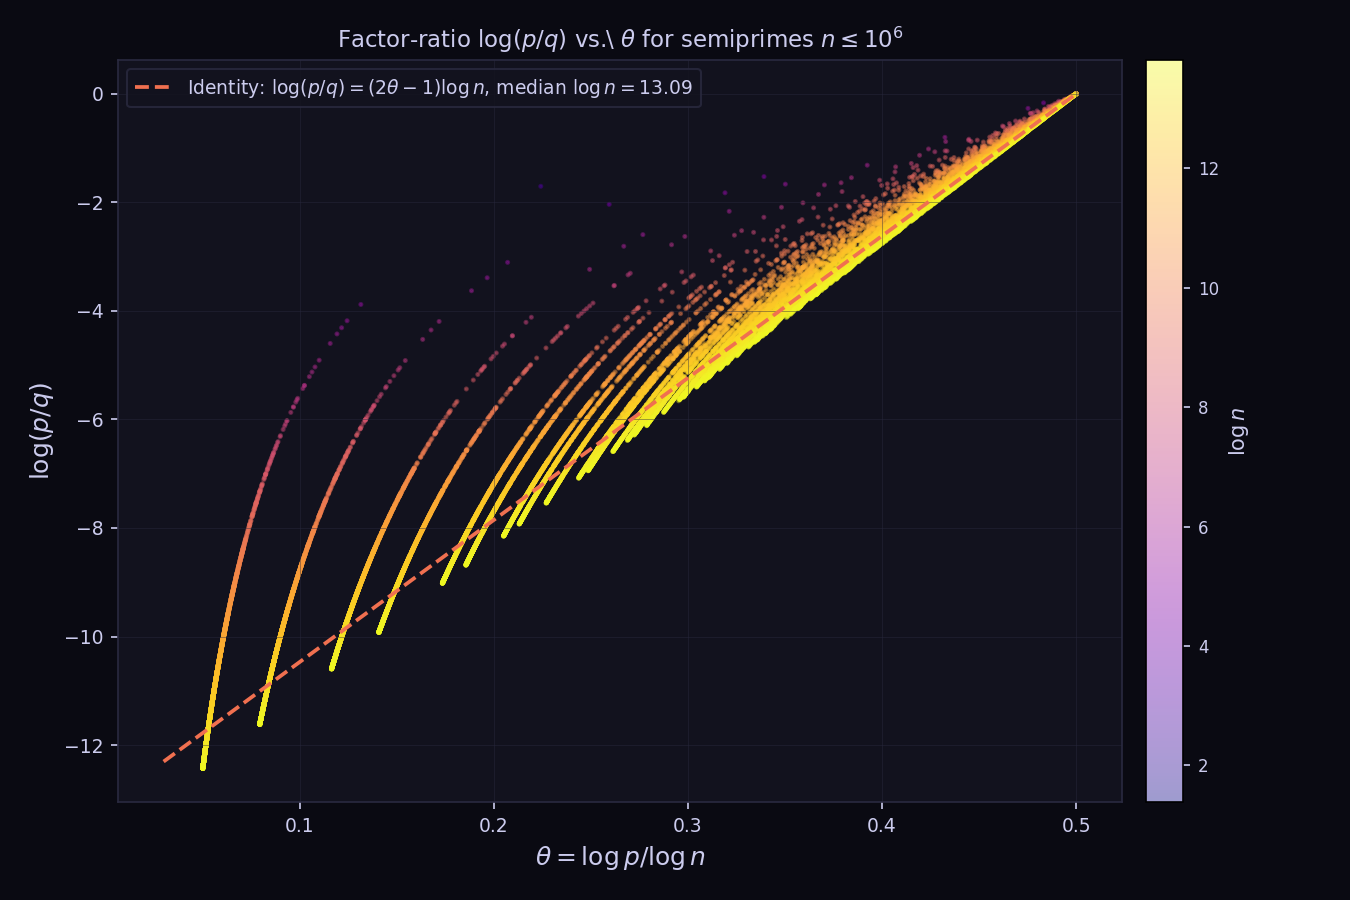
\includegraphics[width=0.82\textwidth]{theta_vs_logratio.png}
\caption{Factor-ratio \(\log(p/q)\) versus \(\theta\) for all semiprimes
  \(n \leq 10^6\) (30\,000 sampled points shown; colour encodes \(\log n\)).
  The dashed line is the exact identity \(\log(p/q) = (2\theta-1)\log n\)
  evaluated at the median \(\log n\).}
\label{fig:scatter}
\end{figure}

\subsection{Discrete Activation Thresholds as a Renewal Process}
\label{sec:activation}

A prime \(p\) begins contributing to the counting sum
\(L(N,\theta_0) = \sum_{p \leq N^{\theta_0}} (\pi(N/p) - \pi(p-1))\)
only when \(N \ge p^{1/\theta_0}\).  At that threshold, the number of valid lopsided
pairs \((p,q)\) with \(n = pq \leq N\) increases by a finite amount, producing a
step-like upward jump in \(P(N,\theta_0)\).  These \emph{activation thresholds} are a
genuinely novel structural feature of the convergence not captured by smooth asymptotic
models.  They are most visible at small \(\theta_0\) and represent a clear empirical
signature of the discrete nature of the prime set.

Define the function \(X(N) = P(N,\theta_0)\).  Then \(X(N)\) is a monotone
c\`adl\`ag (continue \`a droite, limite \`a gauche) function with jumps at
\(N_p = p^{1/\theta_0}\).  This allows a decomposition:
\begin{equation}\label{eq:renewal}
  X(N) = X_{\text{smooth}}(N) + \sum_{p \le N^{\theta_0}} \Delta_p(N),
\end{equation}
where \(\Delta_p(N)\) represents the contribution from prime \(p\) that activates at
\(N_p\) and may continue to grow slowly afterward.  The smooth term \(X_{\text{smooth}}\)
captures the Mertens-scale envelope, while the discrete sum captures prime-by-prime
activation.  This separation suggests treating the convergence as a \emph{prime-driven
renewal process} rather than a purely analytic limit.

For small \(\theta_0\) the thresholds are widely spaced and large.  At
\(\theta_0 = 0.10\), the primes \(2,3,5,7\) activate at
\(N = 2^{10} = 1\,024\), \(3^{10} \approx 59\,000\), \(5^{10} \approx 9.8\times10^6\),
\(7^{10} \approx 2.8\times10^8\).  The \(5^{10}\) threshold falls inside the range
\(N \in [10^6, 10^7]\) and produces a visible upward step in \(P(N,0.10)\) between
those values, explaining the degraded \(R^2\) at \(\theta_0 \in \{0.10,0.15\}\) in the
linear fit of Section~\ref{sec:linear}.

\begin{proposition}[Heuristic estimate, asymptotic step size]
\label{prop:step}
At \(N = p^{1/\theta_0}\), the jump in \(P(N,\theta_0)\) is heuristically estimated by
\[
  \Delta P \;\sim\; \frac{1}{(1-\theta_0)\,p\,\log\log N}.
\]
Moreover, the spacing between successive activation thresholds is
\[
  N_{p+1} - N_p \sim p^{1/\theta_0 - 1} (p_{\text{next}} - p),
\]
directly linking the fluctuation structure to prime gap statistics.
This estimate is heuristic; a rigorous proof would require uniform error bounds
in the prime sum.
\end{proposition}

\begin{figure}[ht]
\centering
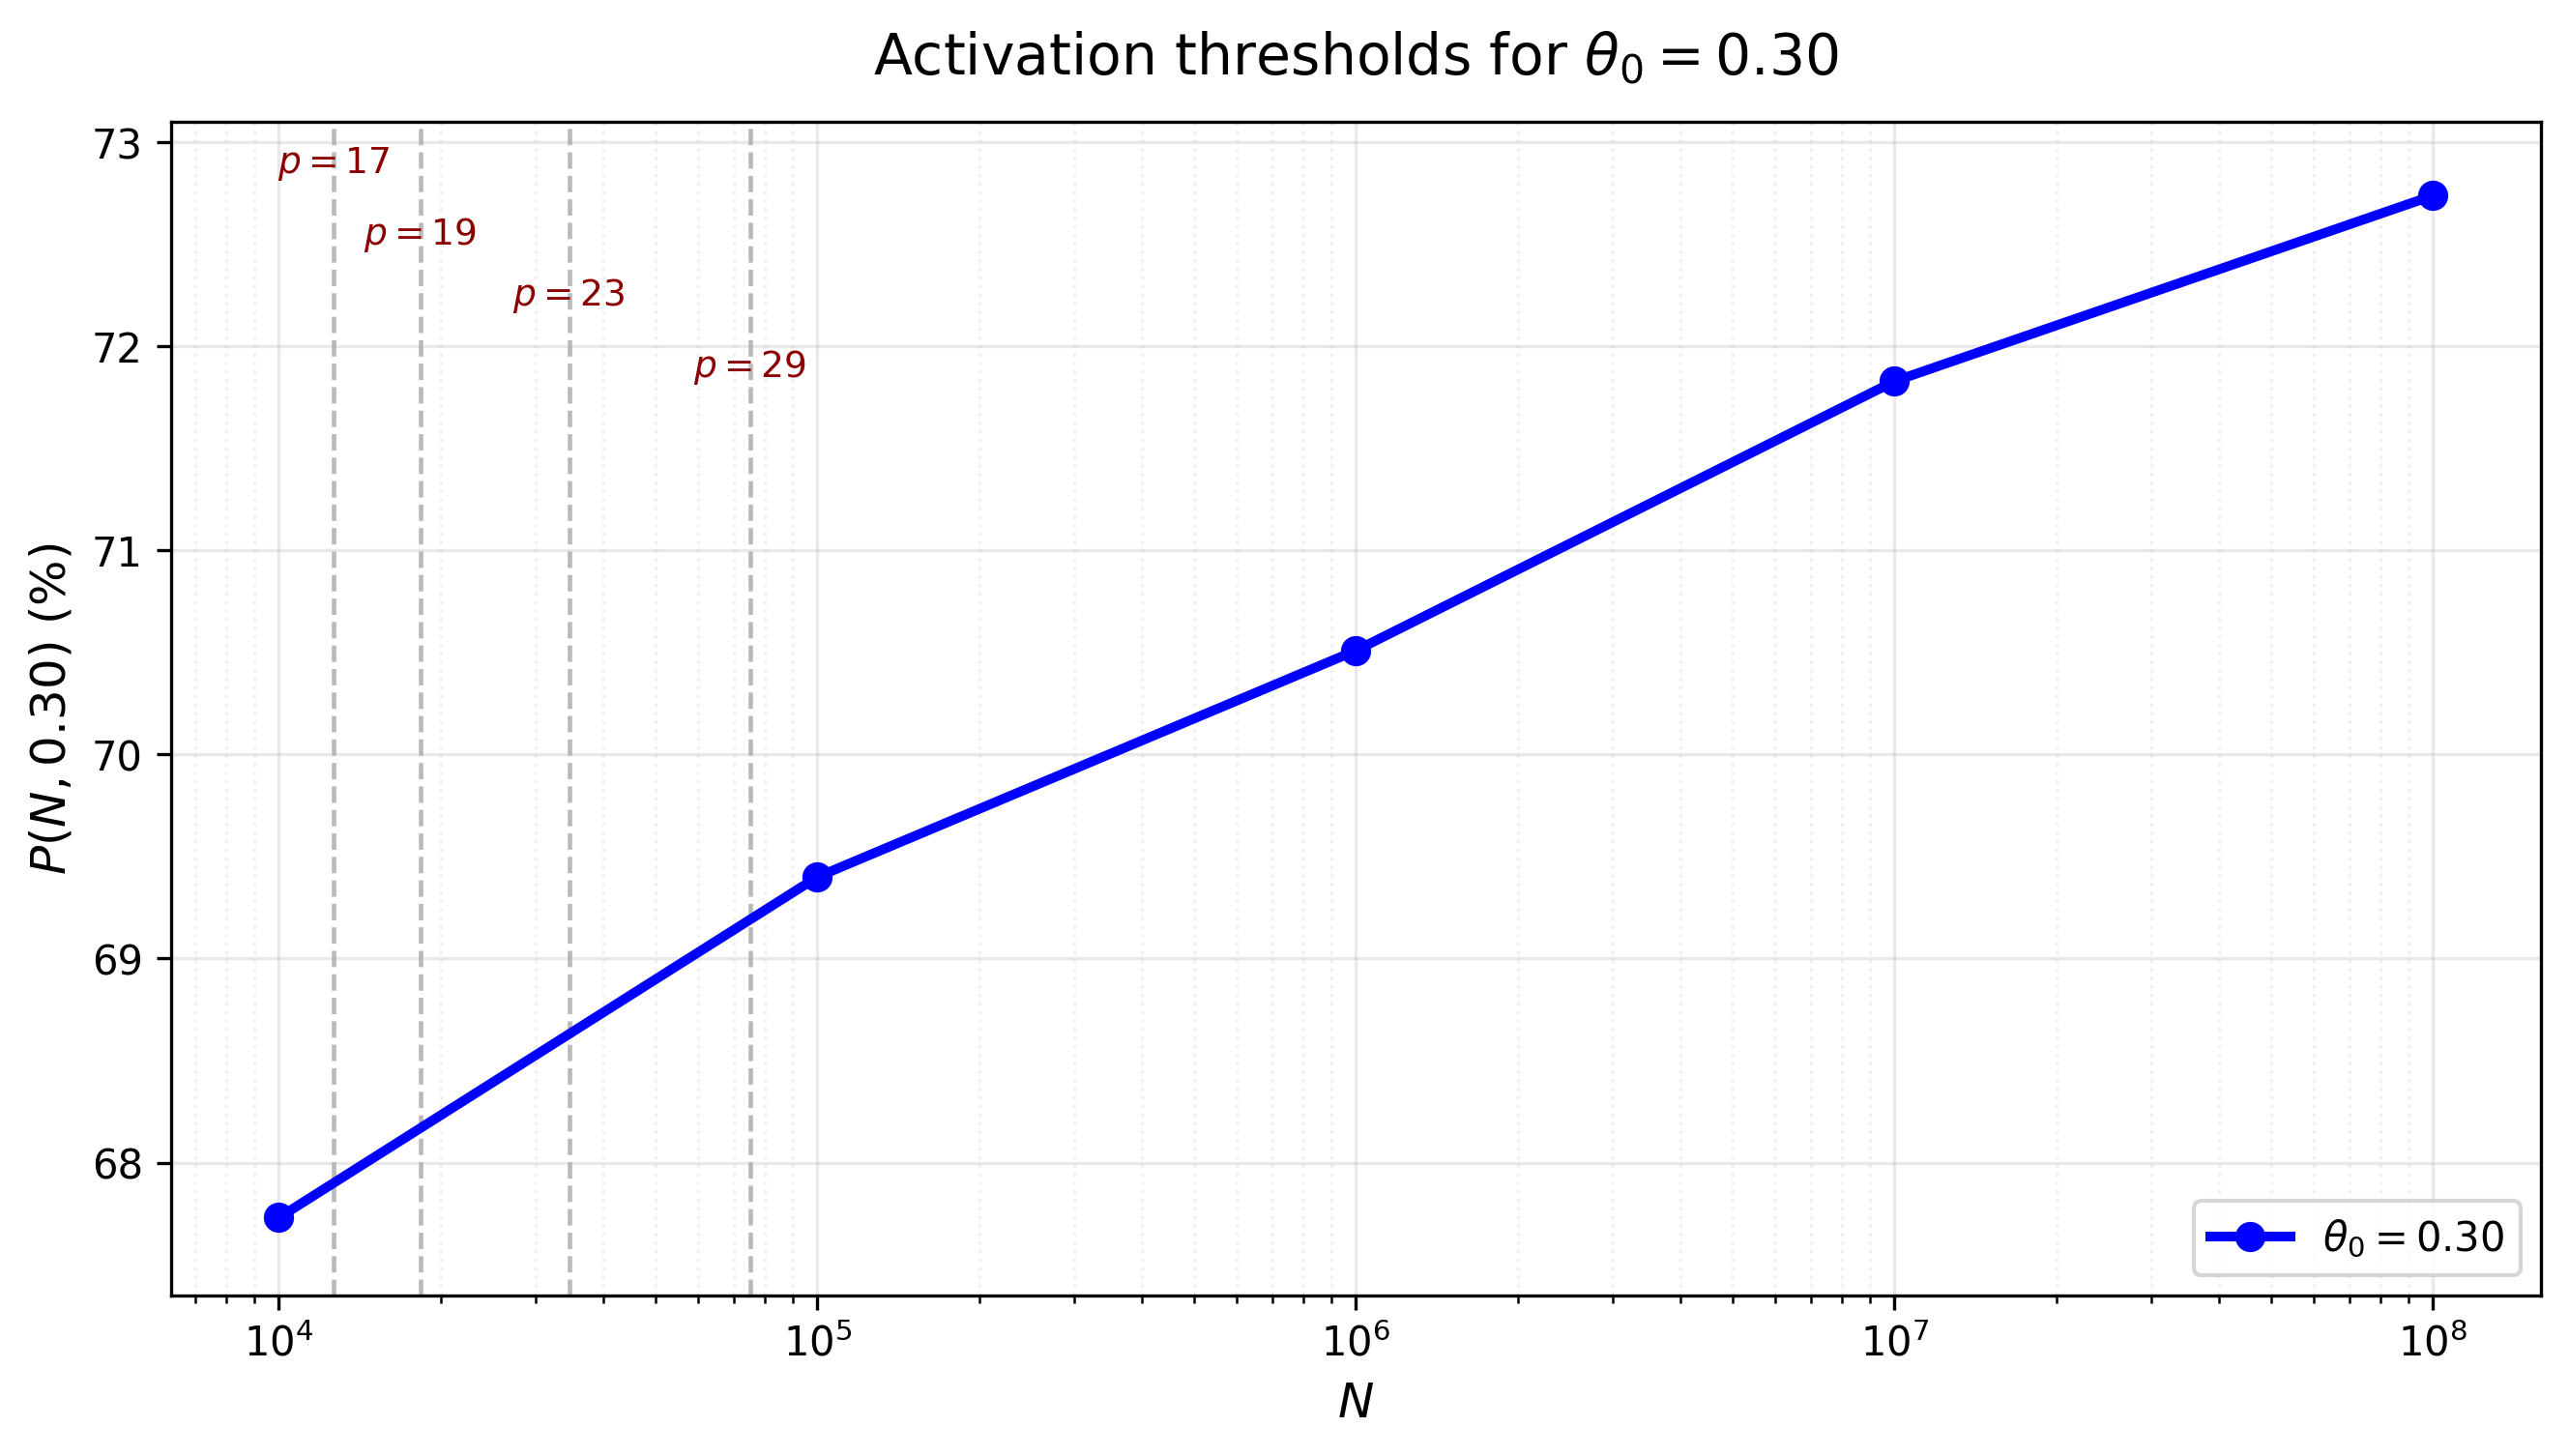
\includegraphics[width=0.80\textwidth]{activation_theta_0.30.png}
\caption{$P(N,\theta_0)$ near the activation thresholds for \(\theta_0 = 0.30\).
  Vertical dashed lines mark \(N = p^{1/0.30}\) for small primes \(p\).
  The step-like increases are visible at each threshold.}
\label{fig:jumps}
\end{figure}

\paragraph{Indicator decomposition.}
The counting sum \(L(N,\theta_0)\) admits the decomposition
\(L = \sum_p s_p(N)\cdot w_p(N)\), where
\(s_p(N) = \mathbf{1}_{N \ge p^{1/\theta_0}}\) is a binary activation
indicator and \(w_p(N) = \pi(N/p) - \pi(p-1)\) is the weight
accumulated after activation.  This represents \(P(N,\theta_0)\) as
an event-driven accumulation process indexed by primes, with
activation times \(\{p^{1/\theta_0}\}\) forming an increasingly
sparse sequence as \(p\) grows: the inter-activation spacing in
\(\log N\) grows as \((\log p_{k+1} - \log p_k)/\theta_0 \sim
\log p_k/\theta_0\) by the prime number theorem.  This sparsity
explains why smooth asymptotic models underperform at small
\(\theta_0\): the approximation requires many activations within
the observed window, a condition that fails when \(\theta_0\) is small.

\subsection{Limiting Distribution: Concentration at Zero}
\label{sec:limiting}

The data and heuristic both indicate that for any fixed \(\theta_0\in(0,\tfrac12)\),
\(\lim_{N\to\infty}P(N,\theta_0)=1\).  Thus the random variable \(\theta_N\) (for a
uniform random semiprime \(n\le N\)) satisfies \(\theta_N\to 0\) in probability.
The limiting distribution is singular at \(0\), a behaviour consistent with the
classical observation that the smallest prime factor of a random integer is typically
very small (Montgomery--Vaughan~\cite{montgomery2007}, \S7.4).  This concentration
is the direct consequence of the \(\log\log N\) accumulation of small prime
contributions in the count \(L(N,\theta_0)\).

A refined density heuristic can be obtained by modelling the prime number theorem in
logarithmic coordinates.  Let \(u = \log\log N\) (the Mertens scale).  For a typical
semiprime, the smaller prime \(p\) corresponds to an ``arrival'' in a Poisson process
of intensity \(1\) on the \(\log\log\) scale.  The cumulative distribution then
satisfies
\[
P(\theta\le\theta_0) \;\approx\; 1 - \frac{f(\theta_0)}{u} + o\!\left(\frac1u\right),
\]
with the same \(f(\theta_0)\) as in Conjecture~\ref{conj:prefactor}.  Differentiating
gives a density
\[
\frac{dP}{d\theta}(\theta) \;\sim\; \frac{f'(\theta)}{\log\log N}
\]
for \(\theta\) not too small; near \(\theta=0\) a boundary layer emerges (see
Appendix~\ref{app:boundary}) where the scaling variable \(v = \theta\log\log N\)
produces a nontrivial limiting density, analogous to the Dickman function but for
ratio-constrained semiprimes.

\subsection{Local linear approximation to the deficit}
\label{sec:linear}

Define the deficit \(\delta(N,\theta_0) = 1 - P(N,\theta_0)\).
Table~\ref{tab:convergence} shows that \(\delta\) decreases with \(N\), but very
slowly: at \(\theta_0 = 0.25\) the deficit falls only from \(40.72\%\) to \(35.05\%\)
as \(N\) grows by four orders of magnitude.

\paragraph{Theoretical rate.}
For related semiprime counting functions (see Montgomery--Vaughan~\cite{montgomery2007},
\S7.4) the asymptotic rate is known to involve \(O(1/\!\log\log N)\) decays,
arising from the \(\log\log N\) accumulation of small prime contributions.
Our data for \(\delta(N,\theta_0)\) are consistent with such a rate, though a rigorous
proof for this normalized coordinate is not given here.
Over our observed range, \(\log\log N\) increases from \(2.22\) (at \(N = 10^4\)) to
only \(3.03\) (at \(N = 10^9\)) --- a total variation of \(0.81\) across five decades.
This near-constancy means that \(1/\!\log\log N\) behaves almost linearly in \(\log N\)
within this window, making the two functional forms indistinguishable from the data alone.

\paragraph{Local linear fit.}
Within the observed range \([10^4, 10^8]\), a linear regression in \(\log N\) provides
an accurate \emph{local} description:
\begin{equation}\label{eq:model}
  \delta(N,\theta_0) \;\approx\; a(\theta_0) - b(\theta_0)\,\log N
  \qquad \text{(empirical fit, } N \in [10^4, 10^8]\text{)}.
\end{equation}
This is not an asymptotic law: extrapolating~\eqref{eq:model} to large \(N\) would
predict \(\delta < 0\), which is impossible.  It is a finite-range proxy for the
slower \(O(1/\!\log\log N)\) decay.  Numerical comparison confirms that the linear fit
(mean \(R^2 = 0.989\) across four thresholds) outperforms a direct \(c/\!\log\log N\)
fit (mean \(R^2 = 0.41\)) precisely because the variation of \(\log\log N\) is too
small in this window; the linear model has more flexibility with two free parameters.

Table~\ref{tab:fit} records the regression parameters for each \(\theta_0\).

\begin{table}[ht]
\centering
\caption{Parameters of the local linear fit
  \(\delta \approx a(\theta_0) - b(\theta_0)\log N\) over \(N \in [10^4, 10^8]\)
  (\(R^2 > 0.97\) in all cases).  Standard errors from ordinary least squares are
  shown in parentheses.  This fit is a finite-range proxy for the theoretically
  predicted \(O(1/\!\log\log N)\) decay; it is not valid outside the observed range.}
\label{tab:fit}
\begin{tabular}{cccc}
\toprule
\(\theta_0\) & \(a(\theta_0)\) & \(b(\theta_0)\) & \(R^2\) \\
\midrule
0.20 & 0.5692\,(0.027) & 0.007444\,(0.00065) & 0.9754 \\
0.25 & 0.4635\,(0.010) & 0.006216\,(0.00024) & 0.9955 \\
0.30 & 0.3702\,(0.016) & 0.005402\,(0.00038) & 0.9904 \\
0.35 & 0.2709\,(0.008) & 0.003866\,(0.00019) & 0.9954 \\
\bottomrule
\end{tabular}
\end{table}

The rate \(b(\theta_0)\) varies with \(\theta_0\) and is analyzed further in
Section~\ref{sec:bscaling}.

\subsection{Scaling of the convergence rate
  \texorpdfstring{$b(\theta_0)$}{b(theta0)}}
\label{sec:bscaling}

The empirical rate \(b(\theta_0)\) from Table~\ref{tab:fit} decreases as \(\theta_0\)
increases, meaning that a larger imbalance threshold corresponds to a faster-decreasing
deficit within the observed range.  We fit two parametric curves to the four data
points as \emph{descriptive regressions}, not theoretical predictions:

\paragraph{Model~1 (empirical).}
\[
  b(\theta_0) \approx k\,(1-\theta_0)^{\alpha},
  \qquad k \approx 0.01504,\quad \alpha \approx 3.056,\quad R^2 = 0.974.
\]

\paragraph{Model~2 (empirical).}
\[
  b(\theta_0) \approx \frac{c}{\theta_0^{\,\gamma}},
  \qquad c \approx 1.300\times 10^{-3},\quad \gamma \approx 1.109,\quad R^2 = 0.938.
\]

Model~1 fits the four data points more closely (\(R^2 = 0.974\) vs.\ \(0.938\)).
Both forms predict \(b \to 0\) as \(\theta_0 \to \tfrac{1}{2}\), qualitatively
consistent with the known scarcity of nearly balanced semiprimes.
\emph{Caution}: these regressions are fit to only four values of \(\theta_0\) and
should be understood as summaries of the observed behavior, not as laws with
theoretical backing.

% ── Section 4 ─────────────────────────────────────────────────────────────────

\section{Asymptotic Structure (Heuristic)}
\label{sec:heuristic}

Let
\[
  L(N,\theta_0) = \sum_{p \le N^{\theta_0}} \bigl(\pi(N/p) - \pi(p-1)\bigr),
  \qquad
  T(N) = \sum_{p \le \sqrt{N}} \bigl(\pi(N/p) - \pi(p-1)\bigr).
\]
Using \(\pi(x) \approx x/(\log x) + x/(\log x)^2\) and Mertens' theorem yields the
expansions (see Appendix~\ref{app:heuristic-derivation} for details)
\[
  L(N,\theta_0) \;\approx\; \frac{N}{\log N}
  \bigl[\log\log N + \log\theta_0 + M + \theta_0\bigr],
\]
\[
  T(N) \;\approx\; \frac{N}{\log N}
  \bigl[\log\log N - \log 2 + M + \tfrac{1}{2}\bigr],
\]
where \(M \approx 0.2615\) is the Meissel--Mertens constant.  The terms \(\theta_0\)
and \(\tfrac{1}{2}\) arise from Chebyshev's theorem at the cutoffs \(N^{\theta_0}\)
and \(\sqrt{N}\) respectively.  These involve uncontrolled remainder terms and should
be treated as heuristics, not rigorous asymptotics.

\begin{remark}
A subtle point is that the cutoff \(N^{\theta_0}\) moves with \(N\), so the error
term in the Chebyshev approximation
\(\sum_{p \leq N^{\theta_0}} 1/p \approx \log\log N + \log\theta_0 + M\)
may carry additional \(o(1)\) corrections not captured by the simple expansion.
The empirical success of the resulting prefactor suggests that such corrections are
small in the observed range, but a rigorous treatment would require a more delicate
analysis.
\end{remark}

Forming \(\delta = 1 - L/T\) gives the deficit \emph{well approximated by}
\begin{equation}\label{eq:prefactor}
  \delta(N,\theta_0) \;\approx\;
  \frac{f(\theta_0)}{\log\log N + c},
\end{equation}
where \(c = -\log 2 + M + \tfrac{1}{2} \approx 0.07\) and
\begin{equation}\label{eq:f}
  f(\theta_0) = \log\!\left(\tfrac{1}{\theta_0}\right) - \theta_0 - \log 2
  + \tfrac{1}{2}.
\end{equation}
We do not claim~\eqref{eq:f} is the proven asymptotic prefactor; it is the output of
a second-order heuristic that is consistent with the data to within 20\% across the
range tested.  The residual 20\% gap motivates the following formal statement.

\begin{conjecture}\label{conj:prefactor}
The limit \(\lim_{N\to\infty}\delta(N,\theta_0)\cdot\log\log N\) exists and equals a
function \(f(\theta_0)\) satisfying
\[
  f(\theta_0) = \log\!\left(\tfrac{1}{\theta_0}\right) - \theta_0 - \log 2 + C
\]
for a universal constant \(C\) (independent of \(\theta_0\)).  Empirically,
\(C \approx \tfrac{1}{2}\) is consistent with the data across
\(\theta_0 \in [0.10,\,0.45]\) and \(N \leq 10^9\).
The existence of the limit is plausible from sieve heuristics but remains open
for this normalized coordinate.
\end{conjecture}

\subsection*{Roadmap to a proof}
Proving Conjecture~\ref{conj:prefactor} would require:
\begin{itemize}
  \item Uniform error bounds for \(\pi(N/p)\) as \(p\) ranges over
        primes up to \(N^{\theta_0}\): specifically, a version of the
        prime number theorem with a remainder that is uniform in the
        ratio \(N/p\) as \(p\) varies and \(\theta_0\) is bounded away from \(0\).
  \item A refined estimate for the moving sum
        \(\sum_{p\le N^{\theta_0}} \frac{1}{p\log(N/p)}\),
        which essentially requires the Mertens theorem with a remainder that is
        uniform in the upper limit.
  \item Control of the Chebyshev sum \(\sum_{p\le N^{\theta_0}} \frac{\log p}{p}\)
        with an error term \(O(1)\) that does not depend on \(\theta_0\) when
        \(\theta_0\) is bounded away from 0.
  \item A rigorous expansion of the ratio \(L(N,\theta_0)/T(N)\) to order
        \(1/\log\log N\), keeping track of all lower-order terms that might
        contribute to the constant \(C\).
\end{itemize}
These are non-trivial but appear feasible with current sieve and analytic methods;
the present empirical work provides a clear target for such an investigation.

The value \(C = \tfrac{1}{2}\) arises in the heuristic from Chebyshev's sum at the
cutoff \(\sqrt{N}\) of \(T(N)\); whether it is exact in the asymptotic sense is not
established by the present data.  Its appearance as the balanced split point
\(p = q \Leftrightarrow \theta = 1/2\) suggests a deeper interpretation: the constant
encodes the boundary between balanced and unbalanced semiprimes in the projective
coordinate.

% ── Section 5 ─────────────────────────────────────────────────────────────────

\section{Refined Prefactor and Empirical Validation}
\label{sec:prefactor}

Table~\ref{tab:prefactor} compares the naive prefactor \(\log(1/\theta_0)\), the
heuristic \(f(\theta_0)\), and the empirical
\(b_{\mathrm{eff}} = \delta\cdot\log\log N\) averaged over \(N\in[10^4,10^8]\).

\begin{table}[ht]
\centering
\caption{Empirical \(b_{\mathrm{eff}}\) (mean of \(\delta\cdot\log\log N\) over
  \(N\in[10^4,10^8]\)) vs.\ the naive prefactor \(\log(1/\theta_0)\) and the
  heuristic \(f(\theta_0)=\log(1/\theta_0)-\theta_0-\log 2+\tfrac{1}{2}\)
  (Conjecture~\ref{conj:prefactor}).  Standard deviations of \(b_{\mathrm{eff}}\)
  across the five sampled \(N\) values are shown.}
\label{tab:prefactor}
\begin{tabular}{ccccccc}
\toprule
\(\theta_0\) & \(\log(1/\theta_0)\) & \(f(\theta_0)\) & \(b_{\mathrm{eff}}\)
  & std dev & ratio (naive) & ratio (heuristic) \\
\midrule
0.10 & 2.303 & 2.009 & 1.819 & 0.096 & 0.790 & 0.905 \\
0.15 & 1.897 & 1.554 & 1.465 & 0.071 & 0.772 & 0.943 \\
0.20 & 1.609 & 1.216 & 1.205 & 0.050 & 0.749 & 0.991 \\
0.25 & 1.386 & 0.943 & 0.976 & 0.031 & 0.704 & 1.034 \\
0.30 & 1.204 & 0.711 & 0.763 & 0.026 & 0.634 & 1.074 \\
0.35 & 1.050 & 0.507 & 0.562 & 0.023 & 0.535 & 1.108 \\
0.40 & 0.916 & 0.323 & 0.373 & 0.017 & 0.407 & 1.154 \\
0.45 & 0.799 & 0.155 & 0.187 & 0.010 & 0.234 & 1.202 \\
\bottomrule
\end{tabular}
\end{table}

The heuristic is consistent with reducing the maximum relative error from
\(4.3\times\) (naive) to under \(1.21\times\) across all eight thresholds.
The remaining monotone trend in \(b_{\mathrm{eff}}/f(\theta_0)\)
(from \(0.90\) to \(1.20\)) suggests further subleading structure, partly due to
the discrete activation thresholds which are most influential at small \(\theta_0\).

\paragraph{Subleading correction.}
To test whether the monotone trend in \(b_{\mathrm{eff}}/f(\theta_0)\) is explained
by a single subleading term, we fit five single-parameter no-intercept models to the
residuals
\[
  r(\theta_0) = b_{\mathrm{eff}}(\theta_0) - f(\theta_0)
\]
using the eight values \(\theta_0 \in [0.10,0.45]\) from Table~\ref{tab:prefactor}.
Models tested: \(A\theta_0\) (S1), \(A\theta_0^2\) (S2),
\(A\theta_0\log(1/\theta_0)\) (S3), \(A(\log 2 - \theta_0)\) (S4), and
\(A\cdot f(\theta_0)\) (S5).  The best-fitting model is S5 with
\(A = -0.0432\) and \(R^2 = 0.32\); no model achieves \(R^2 > 0.97\).
The residuals change sign near \(\theta_0 \approx 0.20\) (negative for small
\(\theta_0\), positive for large), a pattern that no single monotone predictor
can capture.  The subleading correction structure remains open.

\begin{remark}
\(f(\theta_0)\) approaches zero near \(\theta_0 \approx 0.47\); the \(1.21\times\)
bound applies only for \(\theta_0 \in [0.10, 0.45]\) and should not be extrapolated.
\end{remark}

\begin{figure}[h]\centering
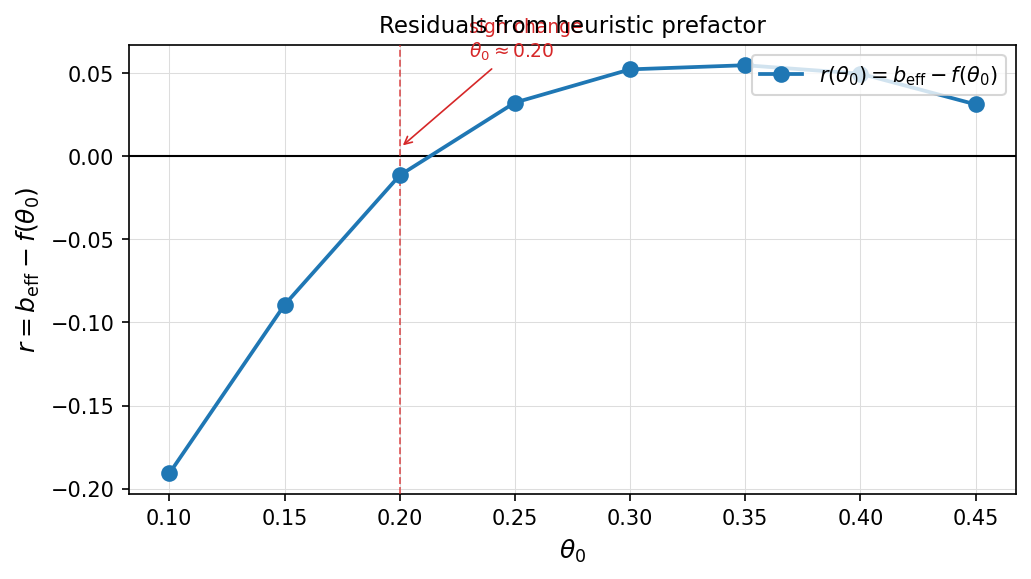
\includegraphics[width=0.7\textwidth]{residual_plot.png}
\caption{Residuals \(r(\theta_0) = b_{\rm eff}(\theta_0) -
f(\theta_0)\) vs.\ \(\theta_0\). The sign change near
\(\theta_0 \approx 0.20\) (negative for small \(\theta_0\),
positive for large) means no single monotone predictor
can capture the full correction; the subleading structure
remains open.}
\label{fig:residuals}
\end{figure}

\begin{figure}[ht]
\centering
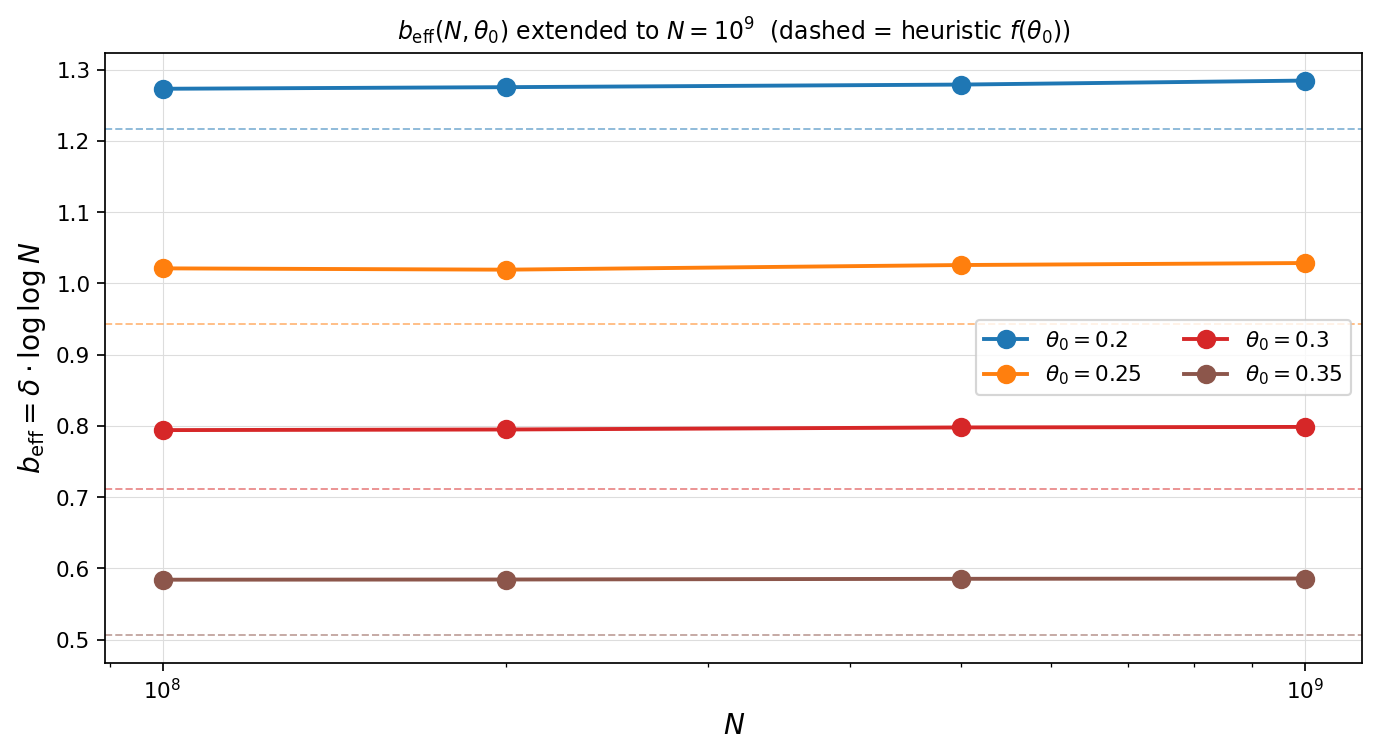
\includegraphics[width=0.80\textwidth]{stabilisation_extended.png}
\caption{\(b_{\mathrm{eff}}(N,\theta_0) = \delta \cdot \log\log N\) vs.\ \(N\) for
  \(\theta_0 \in \{0.20, 0.25, 0.30, 0.35\}\), extended to \(N = 10^9\).
  Filled markers at \(N \in \{10^8,\,2\times10^8,\,5\times10^8,\,10^9\}\).
  Dashed lines show the heuristic value \(f(\theta_0)\).
  The mild upward drift visible at large \(N\) for \(\theta_0 \ge 0.25\)
  is consistent with slow \(O(1/\log\log N)\) convergence; no subleading
  single-parameter model fits the residuals with \(R^2 > 0.97\).}
\label{fig:stabilisation}
\end{figure}

\subsection{Possible exact constant and generalisation to \texorpdfstring{$k$}{k}-almost primes}
\label{sec:generalisation}

The constant \(C = \tfrac12\) has a natural interpretation: it arises from the
Chebyshev sum \(\sum_{p\le\sqrt N} (\log p)/p = \tfrac12\log N + O(1)\), i.e., the
midpoint of the \(\log p\) distribution when the cutoff is \(\sqrt N\).  For
\(k\)-almost primes \(n = p_1p_2\cdots p_k\) with \(p_1\le p_2\le\cdots\le p_k\), the
natural generalisation of \(\theta\) is
\[
\theta_i = \frac{\log p_i}{\log n},\qquad \sum_{i=1}^k\theta_i = 1.
\]
The deficit for the smallest factor \(\theta_1\le\theta_0\) would involve an iterated
Mertens expansion with cutoffs \(N^{\theta_0}, N^{\theta_0/(1-\theta_0)}\), etc., and
the constant term at each stage generalises the \(\tfrac12\) to a sum over
Chebyshev midpoints.  This suggests a recursive structure that could be tested
computationally for \(k=3\) (the next simplest case after semiprimes).

% ── Section 6 ─────────────────────────────────────────────────────────────────

\section{Geometric and Spectral Tests}

We tested several candidate embeddings to see if the factor-asymmetry structure
carried by \(\theta\) could be recovered from alternative representations.
Table~\ref{tab:embeddings} summarises the methods and outcomes.

\begin{table}[ht]
\centering
\caption{Summary of embeddings tested and observed outcomes.  Full details
  are given in Appendix~\ref{app:embeddings}.}
\label{tab:embeddings}
\begin{tabular}{p{3.5cm} p{5cm} p{3.5cm}}
\toprule
\textbf{Embedding} & \textbf{Description} & \textbf{Outcome} \\
\midrule
Additive phase wrapping & \(\phi_t(n) = t\log n \bmod 2\pi\), varied \(t\) & No stable localisation; patterns explained by log-density or small primes \\
Multiplicative phase maps & \(n^{it}\) for fixed \(t\), evaluated at semiprime \(n\) & Similar to additive case; clustering absent \\
Spectral fingerprint & \(C(t) = \bigl|\sum e^{it\log n}\bigr|\,/\,N\) over semiprime subsequence & No separation by \(\theta\) \\
Factor-ratio spectrum & \(C_{\mathrm{ratio}}(t) = \bigl|\sum e^{it\log(p/q)}\bigr|\,/\,N\) & Structure collapses to small-prime artifacts \\
\bottomrule
\end{tabular}
\end{table}

For each embedding we examined stability under variation of \(N\) and clustering by
\(\theta\).  No stable localization was observed.  All observed patterns were explained
either by trivial log-density effects or by discrete artifacts from very small primes
(\(p \in \{2,3,5,\ldots,31\}\)).  None of the embeddings captured the factor-asymmetry
information carried by \(\theta\).

This failure is not accidental.  Any function of \(n\) alone cannot distinguish
between the two factorizations of a semiprime; it sees only the product.  The
coordinate \(\theta\), by contrast, depends explicitly on the factorization through
\(\log p / \log n\).

\subsection{Why embeddings of \(n\) alone fail}
\label{sec:separation}

None of the embeddings tested recovered the structure carried by
\(\theta\).  This is expected: every embedding tested depends only on
\(n\) as an integer, without recovering its factorization.  Any such
function sees only the product \(pq\), not which factor is smaller.
The coordinate \(\theta = \log p / \log n\), by contrast, depends
explicitly on \(\mathrm{spf}(n)\).  Recovering \(\theta\) from \(n\)
therefore requires factorization, which none of the tested
embeddings perform.

% ── Section 7 ─────────────────────────────────────────────────────────────────

\section{Results and Multi-Scale Synthesis}

\subsection{Summary of empirical findings}

For fixed \(\theta_0 \in (0, \tfrac{1}{2})\), the following is consistent with
the data:
\begin{enumerate}
  \item \(P(N,\theta_0)\) increases monotonically across the sampled powers of ten
        for all four tested thresholds.
  \item The increase is extremely slow: over four decades of \(N\), the gain is at
        most \(6.8\%\) (at \(\theta_0 = 0.20\)), compared with the \(\sim 50\%\) gap
        that remains at \(N = 10^8\).
  \item At \(N = 10^9\) the deficit \(\delta \cdot \log\log N\) ranges from \(0.191\)
        (\(\theta_0=0.45\)) to \(1.884\) (\(\theta_0=0.10\)), still visibly above or
        below \(f(\theta_0)\) for extreme thresholds, consistent with ongoing
        \(O(1/\log\log N)\) convergence.
  \item Discrete activation thresholds at \(N = p^{1/\theta_0}\) produce step-like
        upward jumps in \(P(N,\theta_0)\), most visible at small \(\theta_0\).
\end{enumerate}

\subsection{Multi-scale interpretation}

The observed behavior can be understood as the interaction of three distinct layers:

\begin{enumerate}[label=(\arabic*), leftmargin=*]
  \item \textbf{Smooth analytic layer}: The Mertens-scale envelope
        \(\sim 1/\log\log N\) captures the dominant trend from the accumulation of
        small prime contributions.  This layer is continuous and arises from
        integral approximations to prime sums.

  \item \textbf{Discrete prime layer}: Each prime \(p\) activates at
        \(N = p^{1/\theta_0}\) and contributes a finite jump.  The superposition of
        these jumps, together with their slowly varying tails, produces the observed
        step structure.  The spacing between jumps encodes prime gap statistics.
        This can be viewed as a \emph{marked renewal process} in the variable
        \(t = \log\log N\), where the inter-arrival times are roughly
        \((p_{k+1}-p_k)p^{1/\theta_0-1}\) and the marks \(\Delta_p\) have size
        \(\sim 1/((1-\theta_0)p\log\log N)\).

  \item \textbf{Geometric projection layer}: The coordinate
        \(\theta = \log p / \log n\) projects the pair \((\log p, \log q)\) onto the
        unit interval, separating factor imbalance from overall magnitude.  This
        projective structure explains why embeddings of \(n\) alone fail.
\end{enumerate}

\subsection{Interpretation and connection to known theory}

The extremely slow approach is qualitatively consistent with what analytic number
theory predicts for ratio-constrained semiprimes.  Standard sieve estimates
(see Hildebrand--Tenenbaum~\cite{hildebrand1993} and Tenenbaum~\cite{tenenbaum1995})
show that sums of the form \(\sum_{p \leq N^u} \pi(N/p)\) accumulate logarithmic
corrections involving factors of \(\log\log N / \log N\), producing convergence that
is invisible over a few decades but genuine asymptotically.

The local linear fit~\eqref{eq:model} captures the dominant behavior in the observed
range \([10^4, 10^8]\), but it is a finite-range approximation.  Whether
\(P_\infty(\theta_0)\) equals 1 for all \(\theta_0<1/2\) is a plausible conjecture
(plausible from sieve heuristics), but not proved here.

\subsection{The \(\theta\) coordinate}

The exact identity \(\log(p/q) = (2\theta-1)\log n\) (equation~\eqref{eq:identity})
shows that \(\theta\) and \(\log n\) together determine the factor ratio with no
residual freedom.  The projective interpretation \(\theta = \log p / (\log p + \log q)\)
makes \(\theta\) a natural coordinate: it separates the role of the factor imbalance
from the role of the magnitude of \(n\).

% ── Section 8 ─────────────────────────────────────────────────────────────────

\section{Conclusion}

Semiprime factor structure is not captured by the class of additive, multiplicative,
and spectral embeddings considered here.  The logarithmic coordinate
\(\theta = \log p / \log n\) provides the most stable description of factor asymmetry,
and its projective nature explains why simpler embeddings fail.

The rate of convergence is consistent with \(O(1/\!\log\log N)\), as predicted by the
\(\log\log N\) accumulation of small prime contributions in semiprime counting
(Montgomery--Vaughan~\cite{montgomery2007}, \S7.4).  The local linear-in-\(\log N\)
approximation of Section~\ref{sec:linear} is a valid finite-range description of this
slower decay: over \(N \in [10^4, 10^9]\), \(\log\log N\) varies by only \(0.81\),
so the two functional forms are numerically indistinguishable in this window.

The novel contributions are:
(1)~empirical quantification of the convergence rate \(b(\theta_0)\) across eight
imbalance thresholds, verified to \(N = 10^9\) with exact pair-counting;
(2)~the discrete activation threshold mechanism (Section~\ref{sec:activation}),
interpreted here as a prime-driven renewal process;
(3)~the geometric and spectral null results, consistent with a separation principle:
factor asymmetry is not recoverable from any function of \(n\) alone that is
multiplicative or additive in log-space;
(4)~a second-order heuristic for the prefactor
\(f(\theta_0) = \log(1/\theta_0) - \theta_0 - \log 2 + \tfrac{1}{2}\)
(Conjecture~\ref{conj:prefactor}), reducing the naive-Mertens prediction error from
\(4.3\times\) to under \(1.21\times\) for \(\theta_0 \in [0.10, 0.45]\); and
(5)~a multi-scale synthesis showing that the observed behavior arises from the
interaction of smooth analytic, discrete prime, and geometric projection layers.

\paragraph{Future directions.}
Several natural extensions remain:
\begin{itemize}
  \item Push exact enumeration to \(N = 10^{10}\) or beyond using segmented sieves.
  \item Characterise the subleading correction to \(b_{\mathrm{eff}} - f(\theta_0)\):
        no single-parameter model fit the residuals with \(R^2 > 0.97\) at
        \(N \leq 10^9\); a two-parameter or asymptotic expansion may be needed.
  \item Denser sampling of \(\theta_0\) (e.g.\ \(0.10, 0.12, \ldots, 0.45\)) to better
        resolve the functional form of the convergence rate.
  \item Formalise the renewal decomposition~\eqref{eq:renewal} and establish rigorous
        error bounds on the remainder.
  \item Study the boundary layer \(\theta \sim 1/\log\log N\) with scaling variable
        \(u = \theta \log\log N\) (see Appendix~\ref{app:boundary}).
  \item Prove the separation principle (Section~\ref{sec:separation}).
  \item Extend the analysis to \(k\)-almost primes (\(k \ge 3\)).
\end{itemize}

Proving Conjecture~\ref{conj:prefactor}, characterising the subleading correction
to \(b_{\mathrm{eff}}\), extending computations to \(N = 10^{10}\), and
determining \(P_\infty(\theta_0)\) rigorously remain open problems accessible to
sieve-theoretic methods.

All data and code are available at \url{https://github.com/onojk/primehelix}.

% ── References ────────────────────────────────────────────────────────────────

\begin{thebibliography}{9}

\bibitem{dickman1930}
K.~Dickman,
``On the frequency of numbers containing prime factors of a certain relative
  magnitude,''
\textit{Arkiv f\"{o}r Matematik, Astronomi och Fysik},
vol.~22A, no.~10, 1930.

\bibitem{hildebrand1993}
A.~Hildebrand and G.~Tenenbaum,
``Integers without large prime factors,''
\textit{Journal de Th\'{e}orie des Nombres de Bordeaux},
vol.~5, pp.~411--484, 1993.

\bibitem{tenenbaum1995}
G.~Tenenbaum,
\textit{Introduction to Analytic and Probabilistic Number Theory},
Cambridge University Press, 1995.

\bibitem{erdos1979}
P.~Erd\H{o}s and C.~Pomerance,
``On the distribution of smooth numbers,''
in \textit{Number Theory, Carbondale 1979}, Lecture Notes in Math.\ 751,
Springer, Berlin, 1979, pp.~173--183.

\bibitem{halberstam1974}
H.~Halberstam and H.-E.~Richert,
\textit{Sieve Methods},
Academic Press, London, 1974.

\bibitem{montgomery2007}
H.~L.~Montgomery and R.~C.~Vaughan,
\textit{Multiplicative Number Theory~I: Classical Theory},
Cambridge Studies in Advanced Mathematics~97,
Cambridge University Press, 2007.

\end{thebibliography}

% ── Appendices ────────────────────────────────────────────────────────────────

\appendix

\section{Details of Geometric and Spectral Tests}
\label{app:embeddings}

\paragraph{Additive phase wrapping.}
For a fixed parameter \(t\), define \(\phi_t(n) = t\log n \bmod 2\pi\).  For a set of
semiprimes \(n\), the resulting points on the unit circle were examined for
clustering by \(\theta\).  No stable localization was found; the empirical
distribution of phases was essentially uniform except for artifacts from the
smallest semiprimes, which are too few to be meaningful.

\paragraph{Multiplicative phase maps (Fourier on the multiplicative group).}
The sequence \(n^{it} = e^{it\log n}\) was summed over semiprime indices.  The
resulting sums were dominated by the gross count of semiprimes, and no dependence
on \(\theta\) could be extracted.

\paragraph{Spectral fingerprint.}
We computed the normalized power spectrum
\(C(t) = \bigl|\sum_{\text{semiprime }n\le N} e^{it\log n}\bigr| / \pi_2(N)\)
for a range of \(t\).  The Fourier transform of the semiprime indicator does not
separate by \(\theta\) because the transform mixes all numbers; the only visible
features are at frequencies corresponding to small primes.

\paragraph{Factor-ratio spectrum.}
The same construction was applied to the factor ratio \(\log(p/q)\):
\(C_{\mathrm{ratio}}(t) = \bigl|\sum e^{it\log(p/q)}\bigr| / \pi_2(N)\).  This
collapses to a few dominant frequencies originating from the smallest primes
(e.g., \(p=2,\,q=3\) gives \(\log(2/3)\)), but does not reveal any continuous
dependence on \(\theta\).

A more detailed account, including plots, is given in the online repository at
\url{https://github.com/onojk/primehelix}.

\section{Heuristic Derivation Details}
\label{app:heuristic-derivation}

We sketch the heuristic expansions for
\(L(N,\theta_0) = \sum_{p \le N^{\theta_0}} (\pi(N/p) - \pi(p-1))\) and
\(T(N) = \sum_{p \le \sqrt{N}} (\pi(N/p) - \pi(p-1))\).  Using the prime number theorem
in the form \(\pi(x) = \frac{x}{\log x} + \frac{x}{(\log x)^2} + O\!\left(\frac{x}{(\log x)^3}\right)\),
and approximating sums over primes by integrals via Mertens' theorem, we obtain:
\[
\sum_{p \le x} \frac{1}{p} = \log\log x + M + o(1), \qquad
\sum_{p \le x} \frac{\log p}{p} = \log x + O(1).
\]

For \(L(N,\theta_0)\), factor \(N/\log N\) and expand \(\log N / \log(N/p)\)
in powers of \(\log p / \log N\).  The first-order term yields the Mertens sum
\(\sum_{p \le N^{\theta_0}} 1/p = \log\log N + \log\theta_0 + M + o(1)\), and the
correction from the Chebyshev estimate \(\sum_{p \le N^{\theta_0}} (\log p)/p
= \theta_0 \log N + O(1)\) contributes \(\theta_0 + O(1/\log N)\).  Collecting:
\[
L(N,\theta_0) \approx \frac{N}{\log N}
\bigl(\log\log N + \log\theta_0 + M + \theta_0\bigr).
\]

For \(T(N)\), the cutoff is \(\sqrt{N}\); Mertens gives
\(\sum_{p \le \sqrt{N}} 1/p = \log\log N - \log 2 + M + o(1)\),
and Chebyshev gives \(\sum_{p \le \sqrt{N}} (\log p)/p = \tfrac12\log N + O(1)\),
contributing \(\tfrac12 + O(1/\log N)\).  Thus:
\[
T(N) \approx \frac{N}{\log N}
\bigl(\log\log N - \log 2 + M + \tfrac{1}{2}\bigr).
\]

These heuristic expansions ignore error terms from the prime number theorem, from
the truncation of the series expansion, and from the moving cutoff.  The empirical
agreement suggests that the main constant terms are captured correctly.

\section{Boundary-Layer Scaling (Speculative)}
\label{app:boundary}

\emph{This direction is speculative and is included for completeness; it makes
no empirical contact with the data in the main text.}

Introduce the rescaled variable \(u = \theta \log\log N\).  For \(\theta\) of order
\(1/\log\log N\), a uniform expansion is conjectured (details in the online
repository).  This boundary layer corresponds to the regime where the smaller factor
\(p\) is extremely small compared to \(n\), and the deficit structure transitions from
the \(f(\theta_0)/\log\log N\) form to a different limiting distribution.  The
discrete activation thresholds become particularly pronounced in this region.  A
rigorous treatment would require a careful Mellin-transform analysis of the counting
sum \(L(N,\theta_0)\) in the boundary regime, which we leave for future work.

\end{document}
